\section{Controlling for robustness}
\label{sec:intro}
Cyber-Physical Systems (CPS) must withstand a wide range of problems, from bugs in their software to attacks on and failures of their physical sensors.
Under certain error models, like a bounded disturbance on a sensor reading 
%or a wrong transition in the logic
, a CPS can be designed to be robust to that source of error.
In general, however, unforeseen issues can occur. 
To deal with unforeseen problems, at design time, the system must be verified to be \textit{robust} : i.e., not only does it satisfy its design specifications under the known error models, it must satisfy them robustly.
Similarly, at runtime, the system's controller must make decisions that maximize this satisfaction margin, or \textit{robustness}.
This can give a margin of maneuvarability to the system during which it addresses the unforeseen problem.
Since these problems are, by definition, unforeseen and unmodeled and only detected by their effect on the output, the notion of robustness must be computable using only the output behavior of the system.

%ATC_example
\begin{figure}[t]
\centering
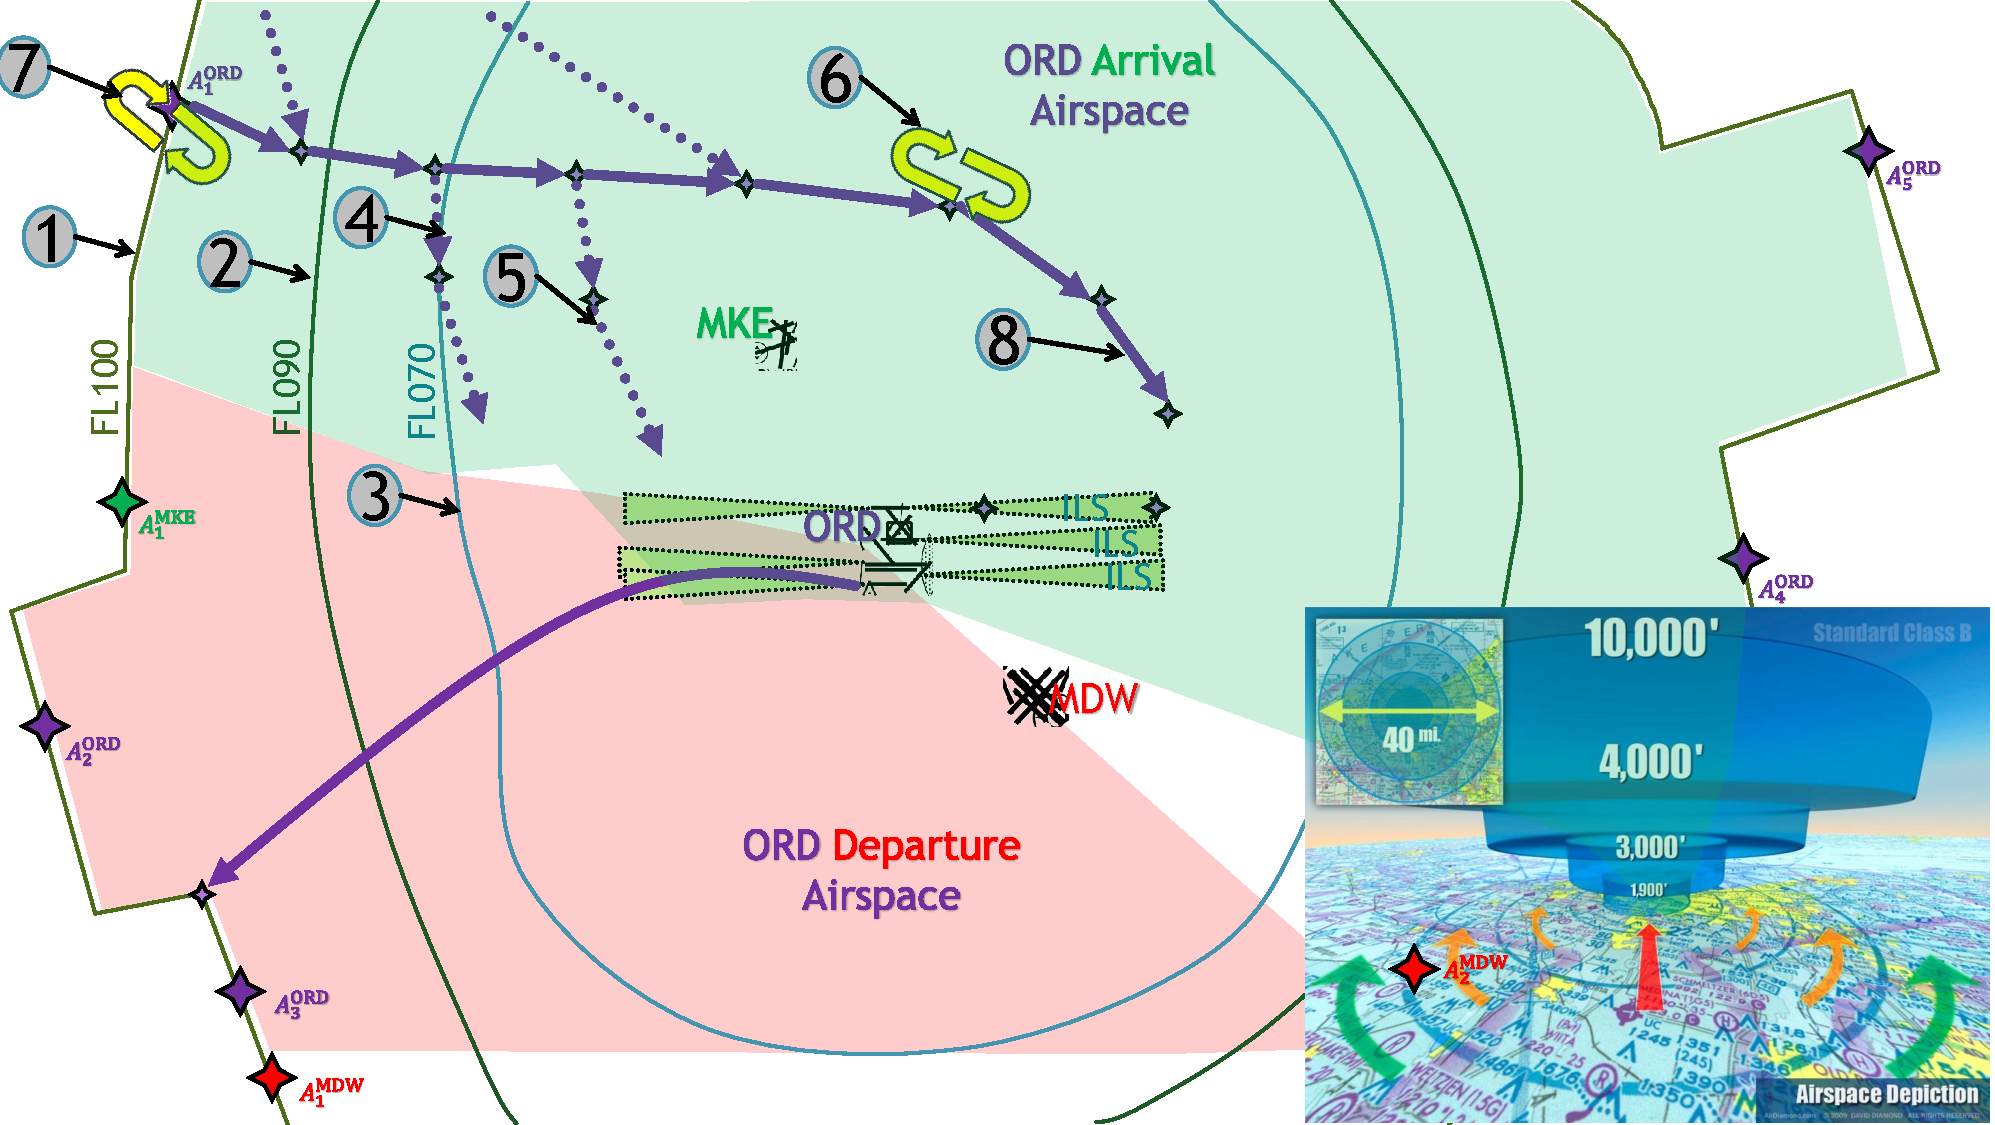
\includegraphics[width=0.49\textwidth]{figures/ATC_Example}
%\vspace{-10pt}
\caption{{\small A simplified depiction of Chicago O'Hare (ORD) airport and its airspace (40 miles radius). The numbers indicate when and where different landing rules apply. Sub-figure on the right shows the altitude rules, see text. Figure courtesy Max Z. Li, Univ. of Pennsylvania.}} 
		%\todo[inline]{Yash, double-check what i wrote in the caption. what is that sub-figure on the right?}}
\label{fig:atc_example}
%\vspace{-20pt}
\end{figure}

\begin{exmp}
%{\sf Example 1: Air Traffic Control}.
Air-Traffic Control (ATC) coordinates landing arrivals at an airport. 
ATCs have very complex rules to ensure that all airplanes, of different sizes and speeds, approach the airport and land safely, \textit{with sufficient margin to other airplanes} to accommodate emergencies and wind gusts.
Fig. \ref{fig:atc_example} depicts the airspace of Chicago O'Hare (ORD), the third busiest airport in the U.S.
The arrival airspace is divided into 3 zones with different, hierarchical, altitude floors and ceilings. 
It also shows holding zones, landing approaches, and allowable trajectories for the landing. 
The following is a subset of the rules that apply for incoming aircrafts.
\end{exmp}

\begin{enumerate}
\vspace{-5pt}
\item When an aircraft enters one of the zones (indicated by the numbers 1,2,3 in Fig.~\ref{fig:atc_example}), it must stay between that zone's altitude floor and ceiling.% E.g. zone 1 has a ceiling of 10,000 feet and a floor of 4000 feet.
\label{rule:floor ceiling}
% of has $1$, $2$ and $3$ mark three Zones, FL100, FL90 and FL70 with altitude ceilings of $10000$, $9000$ and $7000$ feet, and floors of $4000$, $3000$ and $1900$ feet respectively.
\vspace{-5pt}
\item If an aircraft approaches from the West, it must follow one of the trajectories numbered $4$ or $5$. 
%If it approaches from the East (e.g.,  in case of adverse weather), it must follow trajectory $8$.
\label{rule:waypoints}
\vspace{-5pt}
\item If the air-space is too busy, an aircraft must maintain a holding pattern in either holding zones $6$ or $7$, until some maximum amount of time expires.
\label{rule:holding}
% show two holding zones, one at the outer Zone (FL100) and the other in the inner-most zone (FL70). An air-craft could be assigned to a holding zone in case the air-space is too busy.
\vspace{-5pt}
\item A minimum separation must be maintained between aircrafts.
\vspace{-5pt}
\end{enumerate}
\begin{flushright} $\blacksquare$ \end{flushright}

How do we ensure that the ATC system satisfies these complex rules \textit{robustly}?
The \textit{robustness of Metric Temporal Logic specifications} \cite{Fainekos2006_TLVerifSimu,Donze2010} is a rigorous notion that has been used successfully for the verification of automotive systems \cite{Fainekos12_Automotive,Dreossi15_RRTFalsification}, medical devices \cite{SankaranarayananF2012cmsb}, and general CPS.
In details, MTL is a formal language for expressing complex reactive requirements with time constraints, such as those of the ATC~\cite{Koymans90}.
Given a specification $\formula$ written in Metric Temporal Logic (MTL) and a system execution $\sstraj$, the robustness $\robf(\sstraj)$ of the spec relative to $\sstraj$ measures two things:
its sign tells whether $\sstraj$ satisfies the spec ($\robf(\sstraj) > 0$) or falsifies it (i.e., violates it, $\robf(\sstraj) <0$).
Its magnitude $|\robf(\sstraj)|$ measures how \textit{robustly} the spec is satisfied or falsified.
Namely, any perturbation to $\sstraj$ of size less than $|\robf(\sstraj)|$ will not cause its truth value to change.
Thus, the control algorithm can \textit{maximize} the robustness over all possible control actions to determine the next control input.

%\todo[inline]{the font for Example1, continued is different from example 1. see if you can fix this.}
{\sf Example1, continued}.
\textit{The ATC rules can be formalized in Metric Temporal Logic (MTL). Rule \ref{rule:floor ceiling} can be formalized as follows ($\always$ means `Always', $q$ is an aircraft and $q_z$ is its altitude).}
\begin{equation}
\label{eq:rule1mtl}
\always( q \in Zone1 \implies q_z \leq \text{Ceiling1} \land q_z \geq \text{Floor1})
\end{equation}
Rule \ref{rule:holding} can be formalized as follows.
\begin{flalign}
\label{eq:rule3mtl}
\always(Busy \implies\eventually_{[t_1,t_2]} (&q \in \text{Holding-6} \, \lor \,q \in \text{Holding-7}) 
\nonumber \\
&\until_{[0,\text{MaxHolding}]} \neg Busy)
\end{flalign}

\textit{This says that Always ($\always$), if airport is Busy, then Eventually $(\eventually)$, sometime between times $t_1$ and $t_2$, the plane goes into a holding area.
It stays there $\until$ntil the airport is not ($\neg$) busy, or the timer expires at time MaxHolding.} 

\textit{By maximizing the robusness of these MTL specifications, the ATC can automatically find landing patterns that leave room for maneuvering in case of emergencies.}
\textit{Any unforeseen disturbance smaller than a known bounded size will not violate the rules, and will not lead to an unsafe situation.} 
%\vspace{-20pt} \begin{flushright} $\blacksquare$ \end{flushright}


Unfortunately, the robustness function $\robf$ is hard to work with.
It is recursively defined (does not have a closed form), and so is hard to work with analytically.
It is non-convex, so optimizating cannot be guaranteed to yield global optima.
It is non-differentiable, so we have to resort to heuristics or costly nonsmooth optimizers. 
Finally, it does not obey an optimality principle, so efficient Dynamic Programming algorithms cannot be used.
This makes its optimization a challenge - indeed, most existing approaches treat it as a black box and apply heuristics to its optimization (see Related Work below).
These heuristics provide little to no guarantees, have too many user-set parameters, and don't have rigorous termination criteria.
On the other hand, \textit{gradient descent optimization} algorithms typically offer convergence guarantees to the function's (local) minima, have known convergence rates for certain function classes, and have been optimized so they outperform heuristics that don't have access to the objective's gradient information.
The existence of a gradient also allows us to do \textit{local} search for falsifying trajectories, which is necessary for corner case bugs or dangerous situations.
Moreover, gradient descent algorithms usually have a fewer number of parameters to be set by the user, and important issues like step-size selection are rigorously addressed.

\textbf{Contributions}. In this paper, we present smooth (infinitely differentiable) approximations to the robustness function of arbitrary MTL formulae.
This allows us to run powerful and rigorous off-the-shelf gradient descent optimizers.
We show that the smooth approximation is always within a user-defined error of the true robustness, and illustrate the result experimentally.
%\yhl{We demonstrate that optimizing the smooth approximation yields near-minima of the original robustness}.
We demonstrate that the resulting control algorithms, which use gradient descent on the smoothed robustness, performs better than a heuristic like Simulated Annealing optimizing the original, non-differentiable robustness.
We demonstrate the results on a control case study for an autonomous airport traffic controller. Note, our method can also be applied to the falsification problem by minimizing robustness, instead of maximizing it (as for control).
%zutshi_trajectory_2013,

\textbf{Related work.}
Current approaches to optimizing the robustness fall into four categories: 
the use of heuristics like Simulated Annealing and RRTs~\cite{NghiemSFIGP10hscc,AbbasF_HybridSA12,SankaranarayananF2012hscc,Dreossi15_RRTFalsification,Deshmukh15_IterativeApproaches}, 
nonsmooth optimization \cite{AbbasF13acc}, 
Mixed Integer Linear Programming (MILP) \cite{Raman14_MPCSTL}, 
and iterative approximations \cite{AbbasATVA11_LinFalsification,Abbas14_MTLDescent}.
Black-box heuristics are the most commonly used approach: for example, Simulated Annealing~\cite{NghiemSFIGP10hscc}, cross-entropy \cite{SankaranarayananF2012hscc} and RRTs~\cite{Dreossi15_RRTFalsification}.
The clear advantage of these methods is that they do not require any special form of the objective function: they simply need to evaluate it at various points of the search space, and use its value as feedback to decide on the next point to try.
A significant shortcoming is that, unlike gradient descent optimization, they offer little to no guarantees of convergence to local minima, and their convergence rates are often not known. 
They also use many `magical' parameters that are heurstically set and may affect the results significantly, thus requiring more user interaction than desired.
%The same is true of deterministic heuristics \cite{zutshi_trajectory_2013}, albeit they tend to be more transparent to the user and can be better tuned.
%\todo[inline]{look up latest convergence of cross entropy for continuous spaces, genetic algos}
Because the robustness is non-smooth, the work in \cite{AbbasF13acc} developed an algorithm that decreases the objective function along its sub-gradient. 
This involved a series of conservative approximations, and was restricted to the case of safety formulae.
In \cite{Raman14_MPCSTL}, the authors encoded the MTL formula as a set of linear and boolean constraints, and used an MILP solver to solve them.
%The resulting MILP and used a Mixed Integer Linear Program (MILP) has $O(N\cdot|P|)$ binary variables (where $N$ is the number of samples in the trajectory over which we optimize and $|P|$ is the number of predicates, and $O(N\cdot |\formula|)$ continuous variables.
MILPs are NP-hard, and the sophisticated heuristics used to mitigate this make it hard to characterize their runtimes, which is important in control - see examples in \cite{Raman14_MPCSTL}.
The work closest to ours is \cite{AbbasATVA11_LinFalsification,Abbas14_MTLDescent}.
There, the authors considered safety formulas, for which the robustness reduces to the minimum distance between $\sstraj$ and the unsafe set $U$.
By sub-optimally focusing on one point on the trajectory $\sstraj$, they replaced the objective by a differentiable indicator function for $U$ and solved the resulting problem with gradient descent.

By computing fast smooth approximations of robustness, we circumvent most of the above issues and enable real-time control by robustness maximization.


